%приложения
%
% листы A1
% Акт об отсутствии заимствований
% Рецензии
%

\appendix

% команды далее необходимы для того, чтобы нумерация элементов текста в приложениях была корректной.
\renewcommand{\theequation}{\thechapter.\arabic{equation}}
\renewcommand{\thefigure}{\thechapter.\arabic{figure}}
\renewcommand{\thetable}{\thechapter.\arabic{table}}
% -------
\renewcommand{\appendixname}{ПРИЛОЖЕНИЯ}
\def\chaptername{ПРИЛОЖЕНИЕ}
\def\thechapter{\Asbuk{chapter}\unskip}
\renewcommand{\thesection}{\thechapter.\arabic{section}\unskip}
%%%%%%%%%%%%%%%%%%%%%%%%%%%%%%%%%%%%%%%%%%%%%%%%%%%%%%%%%%%%%%%%%%%%%%%%
\addcontentsline{toc}{chapter}{ПРИЛОЖЕНИЯ}
%%%%%%%%%%%%%%%%%%%%%%%%%%%%%%%%%%%%%%%%%%%%%%%%%%%%%%%%%%%%%%%%%%%%%%%%
% ПРИЛОЖЕНИЕ
\fancyhead[C]{\thepage \\ \textbf{\leftmark}}
\fancyfoot[C]{}
%----------------------------------------------------------------
\includepdfset{turn=true,scale=0.85,linktodoc=true,pages=-,pagecommand={\pagestyle{fancy}}}
%----------------------------------------------------------------
\chapter{}\label{ch:apx_a1}

\begin{figure}[H]
    \centering
    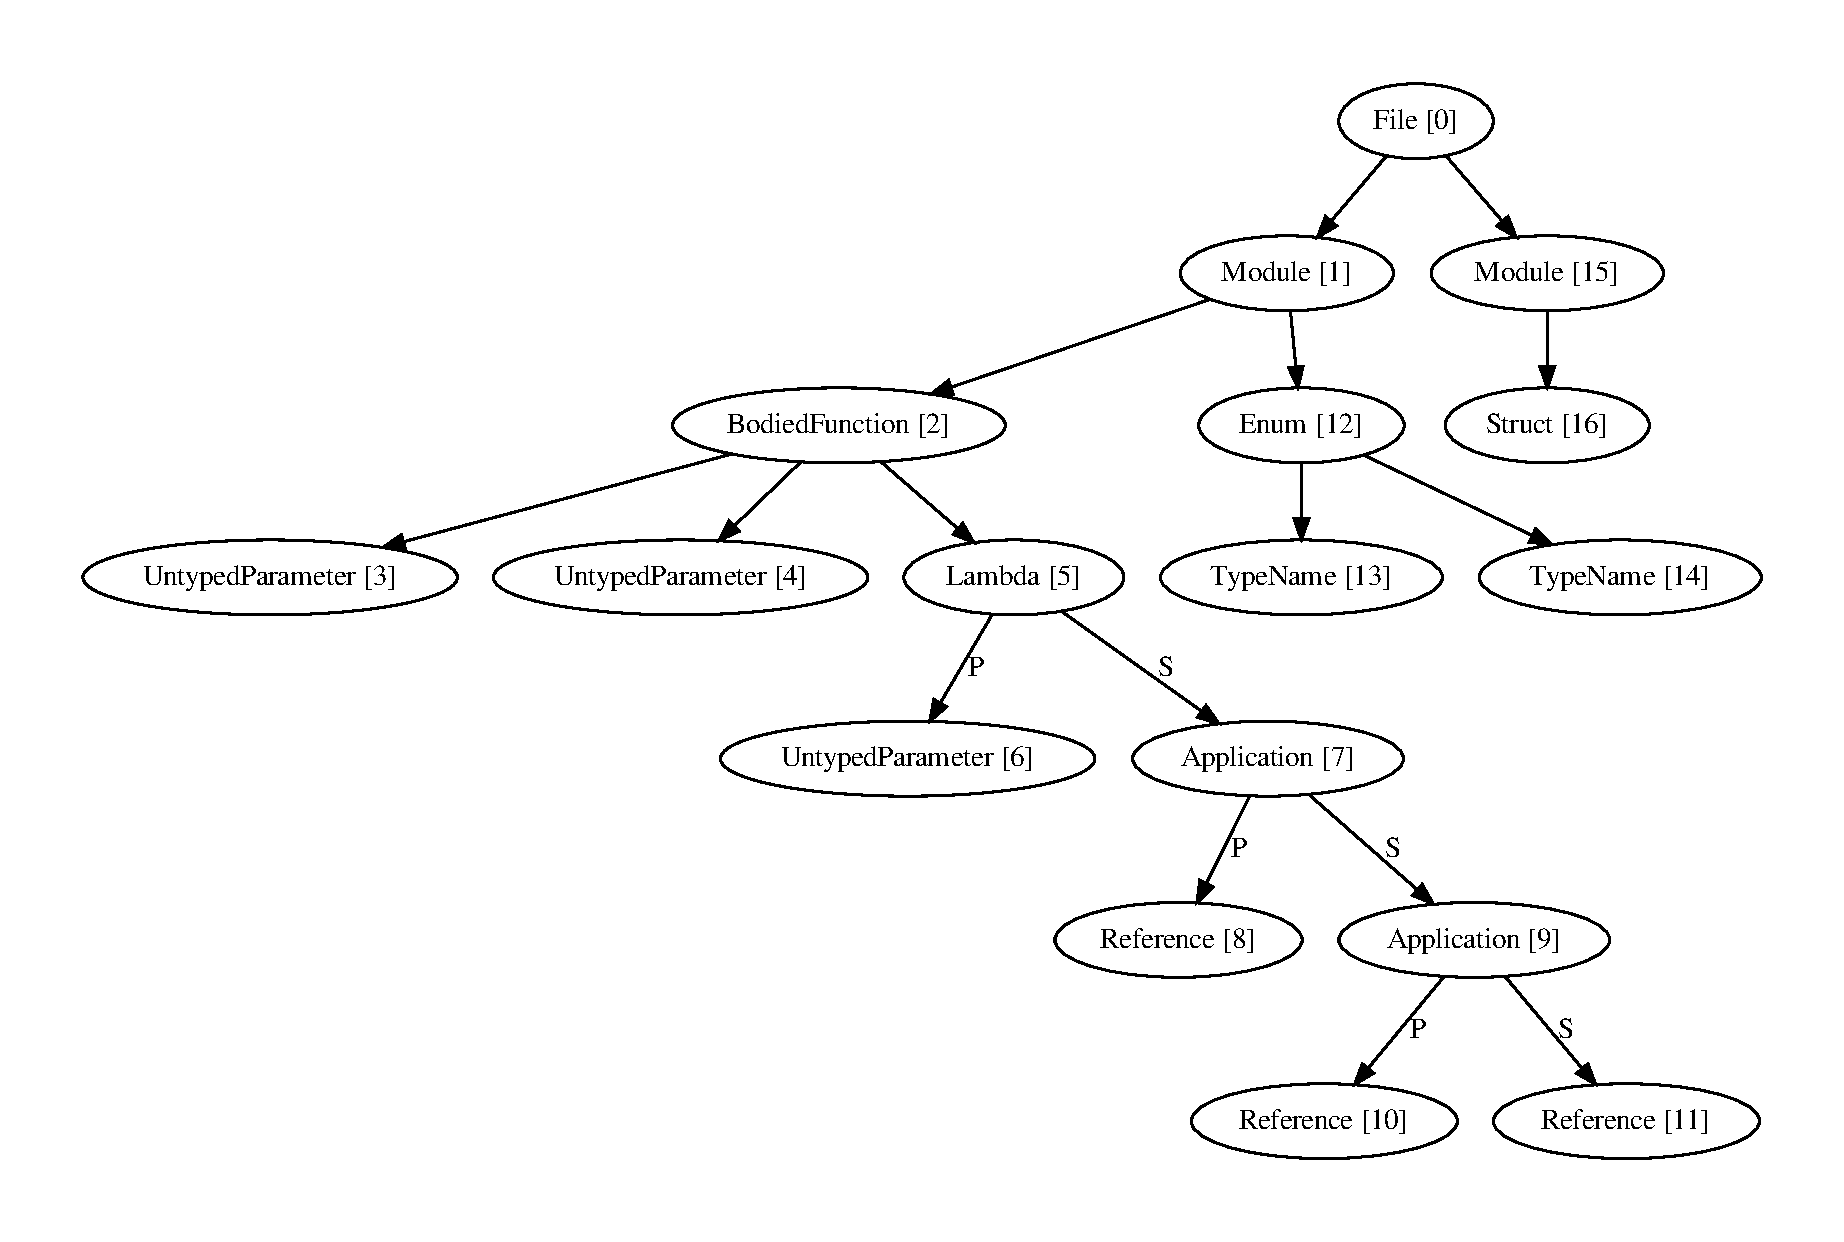
\includegraphics[width=\textwidth]{figures/dot}
    \caption{Изображение структуры абстрактного синтаксического дерева}
    \label{fig:ast_dot}
\end{figure}

\begin{lstlisting}[label=lst:kodept, caption={Исходная программа на языке Kodept}]
module Testing {
    fun compose(f, g) => \x => f(g(x))

    enum struct Bool { True, False }
}

module Testing2 {
    struct Int
}
\end{lstlisting}

\chapter{}\label{ch:apx_b1}

\section*{Элементы абстрактного синтаксического дерева}

\begin{figure}
    \centering
    \input{figures/.generated/ast_nodes}
    \caption{UML-диаграмма }
    \label{fig:ast_nodes}
\end{figure}

%\begin{lstlisting}[label=lst:nodes, caption={Имена всех вершин, составляющих абстрактное синтаксическое дерево}, language=C]
%    File, // root element
%    Module, // module {name} {rest}
%    Struct, // struct {name}({params}) {rest}
%    Enum, // enum {name} {rest}
%    TypedParameter, // {name}: {type}
%    UntypedParameter, // {name}
%    Variable, // val {name}: {type}
%    InitializedVar, // val {name}: {type} = {expr}
%    BodiedFunction, // fun {name}({params}) => {expr}
%    ExpressionBlock, // {  {expr1}; {expr2}; ... }
%    Application, // {expr}({expr})
%    Lambda, // \textbackslash {binds} => {expr}
%    Reference, // {name}
%    Access, // {expr}.{expr}
%    Number, // number literal
%    Char, // char literal
%    String, // string literal
%    Tuple, // ({expr1}, {expr2}, ...)
%    If, // if {expr} => {expr} {другие ветки}
%    Elif, // elif {expr} => {expr}
%    Else, // else {expr}
%    Binary, // binary operator: +, -, *, /, \%, \textasciicircum
%    Unary, // unary operator: -, +, !, \texttildelow
%    AbstractFunction, // abstract fun {name}({params}): {type}
%    ProdType, // ({type1}, {type2}, ...)
%\end{lstlisting}


%{\catcode`\_=11
%\newpage
%\includepdf[pagecommand=\label{appx_A1_list1},pages=-]{appendices/appx_A1_list1.pdf}
%}
%
%%{\catcode`\_=11
%%\newpage
%%\includepdf[pagecommand=\label{appx_A1_list1},pages=-]{appendices/appx_A1_list1.pdf}
%%}
%%----------------------------------------------------------------
%\chapter{Акты и рецензии}\label{apx_acts_reviews}
%
%{\catcode`\_=11
%\newpage
%\includepdf[pagecommand=\label{appx_act_plagiat},pages=-]{appendices/appx_act_plagiatpdf}
%}
%
%{\catcode`\_=11
%\newpage
%\includepdf[pagecommand=\label{appx_review_1},pages=-]{appendices/appx_review_1.pdf}
%}

%%%%%%%%%%%%%%%%%%%%%%%%%%%%%%%%%%%%%%%%%%%%%%%%%%%%%%%%%%%%%%%%%%%%%%%%



